% !TEX root = ../main.tex
\section{Pokročilá teorie ODR - Stabilita, bifurkace a globální vlastnosti}
\label{sec:pokrocila-teorie}

\blocktitle{Cíl kapitoly}
Prohloubit porozumění dlouhodobému a kvalitativnímu chování řešení obyčejných diferenciálních rovnic. Představit metody stability, bifurkací a globálních atraktorů, které propojí lokální teorémy kapitol 1–3 s pokročilými koncepty dynamických systémů a kvantových aplikací.

\begin{intermezzo}
\textbf{Navázání na předchozí kapitoly:} Zatímco Kapitola 3 se zabývala existencí a jednoznačností řešení, nyní studujeme jejich kvalitativní chování pomocí \hyperref[sec:zakladni-teoremy]{teorie stability}, \hyperref[sec:zakladni-teoremy]{bifurkací} a \hyperref[sec:zakladni-teoremy]{globálních vlastností} dynamických systémů.
\end{intermezzo}

\spc

\subsection{Základy teorie stability}

\begin{scaffold}
\item[] \textbf{Co umíme:} Existence, jednoznačnost, Grönwallovo lemma z Kapitoly 3
\item[] \textbf{Co se naučíme:} Definice stability rovnovážných bodů a lokální analýzu  
\item[] \textbf{K čemu to využijeme:} Odhad tolerance systémů vůči rušení, kvantová stabilita
\end{scaffold}

\begin{motivation}
Pochopit, co znamená, že řešení zůstává v okolí rovnovážného stavu. Stabilita je klíčová pro robustnost fyzikálních modelů a spolehlivost technických systémů.
\end{motivation}

\begin{itemize}
\item \textbf{Problém lokální stability:} Chování řešení v okolí rovnovážných bodů
\item \textbf{Problém globální stability:} Dlouhodobé chování všech řešení
\item \textbf{Problém robustness:} Citlivost na perturbace parametrů
\end{itemize}

\begin{definition}[Ljapunovova stabilita]
Rovnovážný bod $y^*$ systému $y' = f(y)$ je \emph{stabilní}, jestliže pro každé $\epsilon > 0$ existuje $\delta > 0$ takové, že
\[
\|y(0) - y^*\| < \delta \Rightarrow \|y(t) - y^*\| < \epsilon \quad \text{pro všechna } t \geq 0
\]
\end{definition}

\begin{figure}[h]
\centering
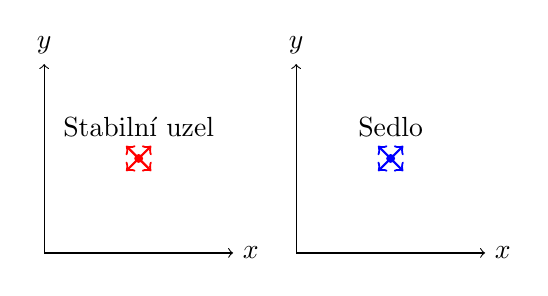
\begin{tikzpicture}[scale=0.8]
% Stabilní uzel
\draw[->] (0,0) -- (3,0) node[right] {$x$};
\draw[->] (0,0) -- (0,3) node[above] {$y$};
\draw[red, thick, ->] (1.5,1.5) -- (1.3,1.3);
\draw[red, thick, ->] (1.5,1.5) -- (1.7,1.3);
\draw[red, thick, ->] (1.5,1.5) -- (1.3,1.7);
\draw[red, thick, ->] (1.5,1.5) -- (1.7,1.7);
\fill[red] (1.5,1.5) circle (2pt);
\node at (1.5,2) {Stabilní uzel};

% Sedlo
\draw[->] (4,0) -- (7,0) node[right] {$x$};
\draw[->] (4,0) -- (4,3) node[above] {$y$};
\draw[blue, thick, ->] (5.5,1.5) -- (5.3,1.3);
\draw[blue, thick, ->] (5.5,1.5) -- (5.7,1.7);
\draw[blue, thick, ->] (5.5,1.5) -- (5.7,1.3);
\draw[blue, thick, ->] (5.5,1.5) -- (5.3,1.7);
\fill[blue] (5.5,1.5) circle (2pt);
\node at (5.5,2) {Sedlo};
\end{tikzpicture}
\caption{Stabilní uzel versus sedlo ve fázovém prostoru}
\label{fig:stability-types}
\end{figure}

\begin{theorem}[Hartman-Grobmanova věta]
Nechť $y^*$ je hyperbolický rovnovážný bod $y' = f(y)$ (žádná vlastní čísla $Df(y^*)$ nemá nulovou reálnou část). Pak existuje homeomorfismus mezi okolím $y^*$ a okolím počátku, který zobrazuje trajektorie nelineárního systému na trajektorie linearizovaného systému $z' = Df(y^*)z$.
\qed
\end{theorem}

\begin{intuition}
V okolí hyperbolického rovnovážného bodu se nelineární systém chová kvalitativně stejně jako jeho linearizace. Stabilní uzel přitahuje trajektorie, sedlo je nestabilní.
\end{intuition}

\begin{keyinsight}
Hartman-Grobmanova věta umožňuje analyzovat lokální stabilitu pomocí linearizace. Pro kvantové systémy to znamená studium spektra Hamiltoniánu kolem stacionárních bodů.
\end{keyinsight}

\begin{summary}
\textbf{Klíčové koncepty:} Ljapunovova stabilita, hyperbolické body, linearizace \\
\textbf{Hlavní výsledky:} Hartman-Grobmanova věta, klasifikace stability \\
\textbf{Aplikace:} Analýza stability kvantových stavů, robustní systémy
\end{summary}

\spc

\subsection{Přímá metoda Ljapunova}

\begin{scaffold}
\item[] \textbf{Co umíme:} Linearizace a stabilita z předchozí sekce
\item[] \textbf{Co se naučíme:} Konstrukci Ljapunovových funkcí a princip invariance  
\item[] \textbf{K čemu to využijeme:} Analýza nelineárních kvantových systémů
\end{scaffold}

\begin{motivation}
Přímá konstrukce funkce, která měří "energii" nebo "vzdálenost" od rovnováhy. Ljapunovova metoda umožňuje analyzovat stabilitu bez explicitního řešení rovnic.
\end{motivation}

\begin{definition}[Ljapunovova funkce]
Funkce $V: D \to \mathbb{R}$ je \emph{Ljapunovova funkce} pro systém $y' = f(y)$ s rovnováhou $y^*$, jestliže:
\begin{itemize}
\item $V(y^*) = 0$ a $V(y) > 0$ pro $y \neq y^*$
\item $\dot{V}(y) = \nabla V(y) \cdot f(y) \leq 0$ na $D$
\end{itemize}
\end{definition}

\begin{theorem}[Ljapunovova věta o stabilitě]
Existuje-li Ljapunovova funkce s $\dot{V}(y) \leq 0$, pak $y^*$ je stabilní. Je-li $\dot{V}(y) < 0$ pro $y \neq y^*$, pak $y^*$ je asymptoticky stabilní.
\qed
\end{theorem}

\begin{example}[Ljapunovova funkce pro nelineární oscilátor]
Pro Duffingův oscilátor $y'' + \delta y' + \alpha y + \beta y^3 = 0$ lze konstruovat Ljapunovovu funkci:
\begin{align*}
V(y,y') &= \frac{1}{2}y'^2 + \frac{\alpha}{2}y^2 + \frac{\beta}{4}y^4 \\
\dot{V}(y,y') &= -\delta y'^2 \leq 0
\end{align*}
což dokazuje stabilitu pro $\delta > 0$.
\end{example}

\begin{application}
\begin{verbatim}
# Python: Numerická verifikace Ljapunovovy stability
def verify_lyapunov(f, V, gradV, equilibrium, domain):
    # Ověření podmínky V(y*) = 0
    assert abs(V(equilibrium)) < 1e-10
    
    # Testování dV/dt ≤ 0 v náhodných bodech
    for _ in range(1000):
        y_test = np.random.uniform(domain[0], domain[1])
        dV_dt = np.dot(gradV(y_test), f(y_test))
        if dV_dt > 1e-10:  # Porušení podmínky
            return False
    return True
\end{verbatim}
\end{application}

\begin{keyinsight}
Ljapunovova metoda umožňuje analyzovat stabilitu komplexních nelineárních systémů, kde linearizace selhává. V kvantových systémech často hraje roli Ljapunovovy funkce Hamiltonián nebo jiné zachovávající se veličiny.
\end{keyinsight}

\begin{summary}
\textbf{Klíčové koncepty:} Ljapunovova funkce, energetické metody \\
\textbf{Hlavní výsledky:} Věty o stabilitě, konstrukce Ljapunovových funkcí \\
\textbf{Aplikace:} Nelineární oscilátory, kvantová stabilita
\end{summary}

\spc

\subsection{Teorie bifurkací}

\begin{scaffold}
\item[] \textbf{Co umíme:} Stabilita a Ljapunovovy metody
\item[] \textbf{Co se naučíme:} Jak se kvalita rovnováh mění s parametry  
\item[] \textbf{K čemu to využijeme:} Kvantové fáze, přechody dynamických režimů
\end{scaffold}

\begin{motivation}
Bifurkace popisují vznik a zánik rovnováh při změně parametrů. Tyto kvalitativní změny odpovídají fázovým přechodům ve fyzikálních systémech.
\end{motivation}

\begin{theorem}[Vidličková bifurkace]
Pro systém $y' = \lambda y - y^3$:
\begin{itemize}
\item $\lambda < 0$: jeden stabilní uzel v $y = 0$
\item $\lambda > 0$: tři rovnováhy - $y = 0$ (sedlo), $y = \pm\sqrt{\lambda}$ (stabilní uzly)
\end{itemize}
\end{theorem}

\begin{theorem}[Hopfova bifurkace]
Nechť $y' = f(y,\lambda)$ má pro $\lambda = \lambda_0$ rovnováhu $y^*$ s vlastními čísly $\alpha(\lambda) \pm i\beta(\lambda)$, kde $\alpha(\lambda_0) = 0$, $\beta(\lambda_0) \neq 0$ a $\frac{d\alpha}{d\lambda}(\lambda_0) \neq 0$. Pak v okolí $\lambda_0$ vzniká limitní cyklus.
\qed
\end{theorem}

\begin{figure}[h]
\centering
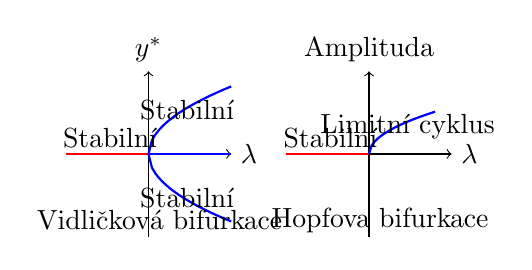
\begin{tikzpicture}[scale=0.7]
% Vidličková bifurkace
\begin{scope}
\draw[->] (-1.5,0) -- (1.5,0) node[right] {$\lambda$};
\draw[->] (0,-1.5) -- (0,1.5) node[above] {$y^*$};
\draw[red, thick] (-1.5,0) -- (0,0);
\draw[blue, thick] (0,0) -- (1.5,0);
\draw[blue, thick, domain=0:1.5] plot (\x, {sqrt(\x)});
\draw[blue, thick, domain=0:1.5] plot (\x, {-sqrt(\x)});
\node at (-0.7,0.3) {Stabilní};
\node at (0.7,0.8) {Stabilní};
\node at (0.7,-0.8) {Stabilní};
\node at (0.2,-1.2) {Vidličková bifurkace};
\end{scope}

% Hopfova bifurkace
\begin{scope}[shift={(4,0)}]
\draw[->] (-1.5,0) -- (1.5,0) node[right] {$\lambda$};
\draw[->] (0,-1.5) -- (0,1.5) node[above] {Amplituda};
\draw[red, thick] (-1.5,0) -- (0,0);
\draw[blue, thick, domain=0:1.2] plot (\x, {0.7*sqrt(\x)});
\node at (-0.7,0.3) {Stabilní};
\node at (0.7,0.5) {Limitní cyklus};
\node at (0.2,-1.2) {Hopfova bifurkace};
\end{scope}
\end{tikzpicture}
\caption{Bifurkační diagramy: vidličková a Hopfova bifurkace}
\label{fig:bifurcation-diagrams}
\end{figure}

\begin{intuition}
Bifurkace představují "větvení" řešení - při překročení kritické hodnoty parametru se systém kvalitativně mění. Vidličková bifurkace vytváří nové rovnováhy, Hopfova bifurkace generuje oscilace.
\end{intuition}

\begin{keyinsight}
Bifurkační teorie poskytuje framework pro pochopení fázových přechodů v kvantových systémech. Kritické body odpovídají hodnotám parametrů, kde se mění kvalitativní chování systému.
\end{keyinsight}

\begin{summary}
\textbf{Klíčové koncepty:} Bifurkační body, kvalitativní změny \\
\textbf{Hlavní výsledky:} Vidličková a Hopfova bifurkace \\
\textbf{Aplikace:} Fázové přechody, vznik oscilací
\end{summary}

\spc

\subsection{Strukturální stabilita}

\begin{scaffold}
\item[] \textbf{Co umíme:} Bifurkace a stabilita
\item[] \textbf{Co se naučíme:} Odolnost dynamiky vůči perturbacím  
\item[] \textbf{K čemu to využijeme:} Robustní návrh kvantových systémů
\end{scaffold}

\begin{motivation}
Určit, kdy je dynamický systém "generický" a odolný vůči malým změnám. Strukturálně stabilní systémy si zachovávají kvalitativní chování při malých perturbacích.
\end{motivation}

\begin{definition}[Strukturální stabilita]
Systém $y' = f(y)$ je \emph{strukturálně stabilní} na kompaktní varietě $M$, jestliže existuje okolí $f$ v $C^1$-topologii takové, že každý systém v tomto okolí je topologicky ekvivalentní $f$.
\end{definition}

\begin{theorem}[Peixotova věta]
Na kompaktní dvourozměrné varietě je generický systém strukturálně stabilní právě tehdy, když:
\begin{itemize}
\item Všechny rovnováhy jsou hyperbolické
\item Všechny periodické orbity jsou hyperbolické  
\item Neexistují homoklinické nebo heteroklinické orbity
\end{itemize}
\qed
\end{theorem}

\begin{intuition}
Strukturálně stabilní systém je "typický" - malé změny nemění topologii fázového portrétu. Nestabilní systémy jsou "výjimečné" a citlivé na perturbace, nacházejí se na bifurkacích.
\end{intuition}

\begin{keyinsight}
Strukturální stabilita zaručuje, že matematické modely zůstávají platné i při nevyhnutelných aproximacích a šumu. V kvantových systémech to znamená robustnost vůči decoherenci a perturbacím.
\end{keyinsight}

\begin{summary}
\textbf{Klíčové koncepty:} Strukturální stabilita, generické vlastnosti \\
\textbf{Hlavní výsledky:} Peixotova věta, klasifikace stability \\
\textbf{Aplikace:} Robustní modely, kvantová odolnost
\end{summary}

\spc

\subsection{Hamiltonovské systémy}

\begin{scaffold}
\item[] \textbf{Co umíme:} Matematický fundament z Kapitol 2–3
\item[] \textbf{Co se naučíme:} Geometrický rámec pro konzervativní systémy  
\item[] \textbf{K čemu to využijeme:} Kvantové Hamiltoniány, symplektická integrace
\end{scaffold}

\begin{motivation}
Hamiltonova formulace zdůrazňuje zachování energie a symplektickou geometrii. Tento přístup je fundamentální pro kvantovou mechaniku a teorii integrabilních systémů.
\end{motivation}

\begin{definition}[Symplektická struktura]
\emph{Symplektická forma} na varietě $M$ je uzavřená nedegenerovaná 2-forma $\omega$. Dvojice $(M,\omega)$ se nazývá \emph{symplektická varieta}.
\end{definition}

\begin{theorem}[Liouville-Arnold]
Pro úplně integrabilní systém jsou invariantní tory dány $F_i = \text{konst.}$ a pohyb na nich je kvaziperiodický.
\qed
\end{theorem}

\begin{intuition}
Symplektická struktura zachovává "fázový objem" - Hamiltonovský tok je kanonickou transformací. Akční proměnné popisují invarianty pohybu, úhlové proměnné fázové posuvy.
\end{intuition}

\begin{application}
\begin{verbatim}
# Python: Symplektická integrace pro Hamiltonovské systémy
def symplectic_euler(q, p, H, dt, steps):
    # Symplektická Eulerova metoda zachovává strukturu
    trajectory = []
    for _ in range(steps):
        # Aktualizace hybnosti pak polohy
        p_new = p - dt * H.dH_dq(q, p)    # ∂H/∂q
        q_new = q + dt * H.dH_dp(q, p_new) # ∂H/∂p
        
        q, p = q_new, p_new
        trajectory.append((q.copy(), p.copy()))
    return trajectory
\end{verbatim}
\end{application}

\begin{keyinsight}
Hamiltonovská struktura je fundamentální pro kvantovou mechaniku - kvantování spočívá v nahrazení Poissonových závorek komutátory. Symplektické integrátory zachovávají tuto strukturu v numerických simulacích.
\end{keyinsight}

\begin{summary}
\textbf{Klíčové koncepty:} Symplektická geometrie, integrabilita \\
\textbf{Hlavní výsledky:} Liouville-Arnoldova věta, kanonické rovnice \\
\textbf{Aplikace:} Kvantová mechanika, nebeská mechanika
\end{summary}

\spc

\subsection{Globální atraktory a dissipativní systémy}

\begin{scaffold}
\item[] \textbf{Co umíme:} Asymptotická stabilita
\item[] \textbf{Co se naučíme:} Existence a struktura globálních atraktorů  
\item[] \textbf{K čemu to využijeme:} Dlouhodobé chování otevřených systémů
\end{scaffold}

\begin{motivation}
V dissipativních systémech řešení konverguje k malému atraktoru. Globální atraktor zachycuje veškeré dlouhodobé chování systému.
\end{motivation}

\begin{definition}[Globální atraktor]
Kompaktní množina $\mathcal{A} \subset X$ je \emph{globálním atraktorem}, jestliže:
\begin{itemize}
\item Je invariantní: $S(t)\mathcal{A} = \mathcal{A}$ pro všechna $t \geq 0$
\item Je atrahující: $\lim_{t\to\infty} \text{dist}(S(t)B, \mathcal{A}) = 0$ pro každou ohraničenou $B \subset X$
\end{itemize}
\end{definition}

\begin{theorem}[Existence globálního atraktoru]
Nechť semigroupa $S(t)$ je spojitá, uniformně kompaktní a existuje ohraničená absorbující množina. Pak existuje globální atraktor.
\qed
\end{theorem}

\begin{figure}[h]
\centering
\begin{tikzpicture}[scale=0.6]
% Lorenzův atraktor - zjednodušená schematická reprezentace
\draw[->] (-3,0) -- (3,0) node[right] {$x$};
\draw[->] (0,-2) -- (0,4) node[above] {$z$};
\draw[->] (135:2) -- (315:2) node[below] {$y$};

% Atraktor jako fraktální struktura
\draw[red, thick, rotate=20] 
    (0,0) .. controls (1,1) and (1.5,0.5) .. (2,2)
    .. controls (1.5,3) and (0.5,2.5) .. (0,2)
    .. controls (-0.5,1.5) and (-1,2) .. (-1.5,1)
    .. controls (-1,0) and (0,0.5) .. (0,0);
    
\draw[red, thick, rotate=-20] 
    (0.5,0.3) .. controls (1.2,1) and (1.7,0.8) .. (2.2,2.2);

\node[red] at (1.5,3.2) {Lorenzův atraktor};
\node at (0,-2.5) {Dimense ≈ 2.06};
\end{tikzpicture}
\caption{Lorenzův atraktor - příklad podivného atraktoru s fraktální strukturou}
\label{fig:lorenz-attractor}
\end{figure}

\begin{intuition}
Globální atraktor je "srdce" dynamického systému - všechny trajektorie se k němu nakonec přiblíží a na něm se odehrává zajímavá dynamika. Fraktální dimenze měří komplexitu této struktury.
\end{intuition}

\begin{keyinsight}
Teorie atraktorů popisuje dlouhodobé chování dissipativních systémů. V kvantových systémech mohou atraktory modelovat stacionární stavy otevřených kvantových systémů interagujících s prostředím.
\end{keyinsight}

\begin{summary}
\textbf{Klíčové koncepty:} Globální atraktor, dissipativní systémy \\
\textbf{Hlavní výsledky:} Věty o existenci, fraktální dimenze \\
\textbf{Aplikace:} Chaotické systémy, kvantová optika
\end{summary}

\spc

\subsection{Ergodická teorie dynamických systémů}

\begin{scaffold}
\item[] \textbf{Co umíme:} Globální chování systémů
\item[] \textbf{Co se naučíme:} Statistickou vlastnost trajektorií  
\item[] \textbf{K čemu to využijeme:} Kvantová ergodicita, statistická mechanika
\end{scaffold}

\begin{motivation}
Ergodická teorie propojuje dlouhodobé časové průměry s prostorovými průměry. To je fundamentální pro statistickou mechaniku a kvantovou teorii chaosu.
\end{motivation}

\begin{definition}[Ergodický systém]
Dynamický systém $(X, \mathcal{F}, \mu, T)$ je \emph{ergodický}, jestliže každá $T$-invariantní množina má míru 0 nebo 1.
\end{definition}

\begin{theorem}[Birkhoffův ergodický teorém]
Je-li $f \in L^1(X,\mu)$, pak pro skoro všechna $x \in X$ platí:
\[
\lim_{n \to \infty} \frac{1}{n} \sum_{k=0}^{n-1} f(T^k x) = \int_X f\, d\mu
\]
\qed
\end{theorem}

\begin{example}[Bernoulliho posuv jako mixing systém]
Pro Bernoulliho posuv na $\{0,1\}^\mathbb{Z}$ s mírou $\mu(\{0\}) = \mu(\{1\}) = \frac{1}{2}$ platí:
\[
\lim_{n \to \infty} \mu(T^{-n}A \cap B) = \mu(A)\mu(B)
\]
což dokazuje mixing - silnější vlastnost než ergodicita.
\end{example}

\begin{intuition}
Ergodicita znamená, že "časový průměr = prostorový průměr". Jedna typická trajektorie prozkoumá celý fázový prostor rovnoměrně. Mixing znamená, že korelace mezi stavy v čase mizí.
\end{intuition}

\begin{keyinsight}
Ergodická teorie poskytuje matematický základ pro statistickou mechaniku. V kvantových systémech ergodicita vysvětluje, proč izolované systémy dosahují tepelné rovnováhy a proč vlastní funkce chaotických systémů jsou equidistribuované.
\end{keyinsight}

\begin{summary}
\textbf{Klíčové koncepty:} Ergodicita, mixing, časové průměry \\
\textbf{Hlavní výsledky:} Birkhoffův teorém, vlastnosti mixing \\
\textbf{Aplikace:} Statistická mechanika, kvantová ergodicita
\end{summary}

\spc

\subsection*{Shrnutí kapitoly}

\begin{itemize}
\item Představili jsme pokročilé metody analýzy stability dynamických systémů
\item Ljapunovova metoda umožňuje studovat stabilitu bez explicitního řešení
\item Teorie bifurkací klasifikuje kvalitativní změny při variaci parametrů
\item Strukturální stabilita charakterizuje robustnost dynamiky
\item Hamiltonovská mechanika poskytuje geometrický framework pro konzervativní systémy
\item Teorie atraktorů popisuje dlouhodobé chování dissipativních systémů
\item Ergodická teorie spojuje časové a prostorové středování
\end{itemize}

\vspace{0.5cm}

\begin{tcolorbox}[title=\textbf{Doporučená literatura}, colback=blue!5!white, colframe=blue!75!black]
\begin{itemize}
\item \textbf{Arnold, V. I.} \emph{Mathematical Methods of Classical Mechanics}
\item \textbf{Guckenheimer, J.; Holmes, P.} \emph{Nonlinear Oscillations, Dynamical Systems, and Bifurcations of Vector Fields}  
\item \textbf{Katok, A.; Hasselblatt, B.} \emph{Introduction to the Modern Theory of Dynamical Systems}
\item \textbf{Temam, R.} \emph{Infinite-Dimensional Dynamical Systems in Mechanics and Physics}
\end{itemize}
\end{tcolorbox}

\begin{transition}
V následující kapitole rozšíříme naše porozumění na parciální diferenciální rovnice, kde infinite-dimenzionální povaha problémů vyžaduje sofistikovanější matematický aparát a přináší nové kvalitativní jevy jako disperzi, difúzi a vlnové jevy.
\end{transition}

\spc